% \documentclass[handout,xcolor=pdftex,dvipsnames,table]{beamer}
%\documentclass{beamer}



%支持notes自动生成,分别设置参数“notes”,“notesonly”,分别对照为生成slides+notes模式,和只生成notes模式。
\documentclass[CJKutf8, 10pt, notes]{beamer}
\usetheme[framenumber]{WISE}

% Packages:
% \usepackage{import}
% \usepackage[dutch]{babel}

%添加中文支持,方便中英文进行切换操作。
\usepackage{CJKutf8}
%生成随机文本
\usepackage{lipsum}
%识别千分号
\usepackage{textcomp}

% The title information
\title[]{Example Title}
\subtitle{Example Subtitle}
\author{杨阳}
\institute{厦门大学 王亚南经济研究院}
\date{\today}


% What is this for? (used when including existing pdf slides?)
\setbeamercolor{background canvas}{bg=}

%设定pause后item阴影显示
\setbeamercovered{transparent}

% Remove the navigation symbols
\beamertemplatenavigationsymbolsempty 

% Customise the outline pages
\AtBeginSection[]  
  {  
    \begin{frame}<*>{beamer} 
      \frametitle{概要}
      \tableofcontents[currentsection,currentsubsection]  
    \end{frame}  
  }

\AtBeginSubsection[]
{
  \begin{frame}<*>{beamer} 
    \frametitle{概要}
    \tableofcontents[currentsection,currentsubsection]
  \end{frame}
}

%%%%%%%%%%%%%%%%%%%%%%%%%%%%%%%%%%%%%%%%%%%%%%%%%%%%%%%%%%%%%%%%%%%%%%%%%%%%%%%%%%%%%%%%%%
\begin{document}
\begin{CJK}{UTF8}{gbsn}
\maketitle
%%%%%%%%%%%%%%%%%%%%%%%%%%%%%%%%%%%%%%%%%%%%%%%%%%%%%%%%%%%%%%%%%%%%%%%%%%%%%%%%%%%%%%%%%%

%%%%%%%%%%%%%%%%%%%%%%%%%%%%%%%%%%%%%%%%%%%%%%%%%%%%%%%%%%%%%%%%%%%%%%%%%%%%%%%%%%%%%%%%%%
\section{背景}
 \note{Here you can write some notes.\\
 \lipsum[1]}
%%%%%%%%%%%%%%%%%%%%%%%%%%%%%%%%%%%%%%%%%%%%%%%%%%%%%%%%%%%%%%%%%%%%%%%%%%%%%%%%%%%%%%%%%%

\begin{frame} 
\frametitle{背景}
\begin{alertblock}{Theory}
\lipsum[2]
 \end{alertblock}
 \note{Another note\\
 \lipsum[1]}
%\begin{center}
%  \includegraphics[width=0.4\textwidth]{images/placeholder.jpg}
%\end{center}
\end{frame}

%%%%%%%%%%%%%%%%%%%%%%%%%%%%%%%%%%%%%%%%%%%%%%%%%%%%%%%%%%%%%%%%%%%%%%%%%%%%%%%%%%%%%%%%%%

\begin{frame}
\frametitle{原因}
% \begin{theorem}[Pythagoras]
%  The square of the hypotenuse of a \alert{right} triangle is equal to the sum of the squares on the other two sides:
%  \[
%   a^2 + b^2 = c^2.
%   \]
%    \[\frac{1}{\sigma}\]
%  \end{theorem}
%\begin{proof}
% Straightforward.
%\end{proof}
\pause
\begin{alertblock} {Theory one}
\note<2>{\lipsum[5]}
 \begin{itemize}
 \pause
 \item Reason one

 \pause
 \item Reason two

 \end{itemize}
 \end{alertblock}
 \pause
 \begin{alertblock}{Theory two}

 \begin{itemize}
 \pause
 \item Reason one
 \pause
 \item Reason two
 \pause
 \item  Reason three

\end{itemize}
\end{alertblock}
\end{frame}



%%%%%%%%%%%%%%%%%%%%%%%%%%%%%%%%%%%%%%%%%%%%%%%%%%%%%%%%%%%%%%%%%%%%%%%%%%%%%%%%%%%%%%%%%%
\section{方法}
%%%%%%%%%%%%%%%%%%%%%%%%%%%%%%%%%%%%%%%%%%%%%%%%%%%%%%%%%%%%%%%%%%%%%%%%%%%%%%%%%%%%%%%%%%
\subsection{Method one}
%%%%%%%%%%%%%%%%%%%%%%%%%%%%%%%%%%%%%%%%%%%%%%%%%%%%%%%%%%%%%%%%%%%%%%%%%%%%%%%%%%%%%%%%%%

\begin{frame} 
\frametitle{Method one}
  \begin{itemize}
  \item one

  \pause
  \item two
  \pause
  \item three
  \end{itemize}
 
\end{frame}
%%%%%%%%%%%%%%%%%%%%%%%%%%%%%%%%%%%%%%%%%%%%%%%%%%%%%%%%%%%%%%%%%%%%%%%%%%%%%%%%%%%%%%%%%%
\subsection{Method two}
%%%%%%%%%%%%%%%%%%%%%%%%%%%%%%%%%%%%%%%%%%%%%%%%%%%%%%%%%%%%%%%%%%%%%%%%%%%%%%%%%%%%%%%%%%
\begin{frame} 
\frametitle{Method two}
\begin{definition}
\lipsum[3]
\end{definition}
\end{frame}


%%%%%%%%%%%%%%%%%%%%%%%%%%%%%%%%%%%%%%%%%%%%%%%%%%%%%%%%%%%%%%%%%%%%%%%%%%%%%%%%%%%%%%%%%%
\subsection{Example}
%%%%%%%%%%%%%%%%%%%%%%%%%%%%%%%%%%%%%%%%%%%%%%%%%%%%%%%%%%%%%%%%%%%%%%%%%%%%%%%%%%%%%%%%%%

\begin{frame}
\frametitle{Example}
\begin{table}[!htb] \centering 
 \footnotesize 
\begin{tabular}{@{\extracolsep{5pt}} c c c c } 
\\[-1.8ex]\hline 
\hline \\[-1.8ex] 
Year & Area & Area & Yunnan\\ 
\hline \\[-1.8ex] 
1955&$17,006.520$ & $9,765.123$ & $1,528.830$ \\ 
1956&$19,365.100$ & $9,851.011$ & $1,665.146$ \\ 
1957&$18,021.270$ & $9,746.312$ & $1,585.625$ \\ 
1958&$17,605.080$ & $9,051.152$ & $1,434.889$ \\ 
1959&$19,109.910$ & $9,183.672$ & $1,461.186$ \\ 
1960&$19,568.230$ & $10,809.010$ & $1,334.571$ \\ 
1961&$19,781.670$ & $11,467.330$ & $1,289.073$ \\ 
\hline \\[-1.8ex] 
\normalsize 
\end{tabular} 

  \label{example} 
\end{table} 

\end{frame}

%%%%%%%%%%%%%%%%%%%%%%%%%%%%%%%%%%%%%%%%%%%%%%%%%%%%%%%%%%%%%%%%%%%%%%%%%%%%%%%%%%%%%%%%%%

\begin{frame}
\frametitle{Regression}
\begin{table}[!htb] \centering 
\tiny


\begin{tabular}{@{\extracolsep{5pt}}lc} 
\\[-1.8ex]\hline 
\hline \\[-1.8ex] 
 & \multicolumn{1}{c}{\textit{Dependent variable:}} \\ 
\cline{2-2} 
\\[-1.8ex] & y \\ 
\hline \\[-1.8ex] 
Area1  & $0.456^{***}$ \\ 
  & $(0.009)$ \\ 
  & \\ 
Area2  & $0.123^{***}$ \\ 
  & $(0.032)$ \\ 
  & \\ 
 Constant & $1111.11^{**}$ \\ 
  & $(437.740)$ \\ 
  & \\ 
\hline \\[-1.8ex] 
Observations & $7$ \\ 
R$^{2}$ & $0.895$ \\ 
Adjusted R$^{2}$ & $0.842$ \\
Residual Std. Error & $35.027 (df = 4)$ \\ 
F statistic & $16.966^{**} (df = 2; 4)$ \\ 
\hline 
\hline \\[-1.8ex] 
\textit{Note:}  & \multicolumn{1}{r}{$^{*}$p$<$0.1; $^{**}$p$<$0.05; $^{***}$p$<$0.01} \\ 
\normalsize 
\end{tabular} 

  \label{yunnanReg} 
\end{table} 



\end{frame}

%%%%%%%%%%%%%%%%%%%%%%%%%%%%%%%%%%%%%%%%%%%%%%%%%%%%%%%%%%%%%%%%%%%%%%%%%%%%%%%%%%%%%%%%%%

\begin{frame}
\frametitle{Plot Example}
\begin{center}

 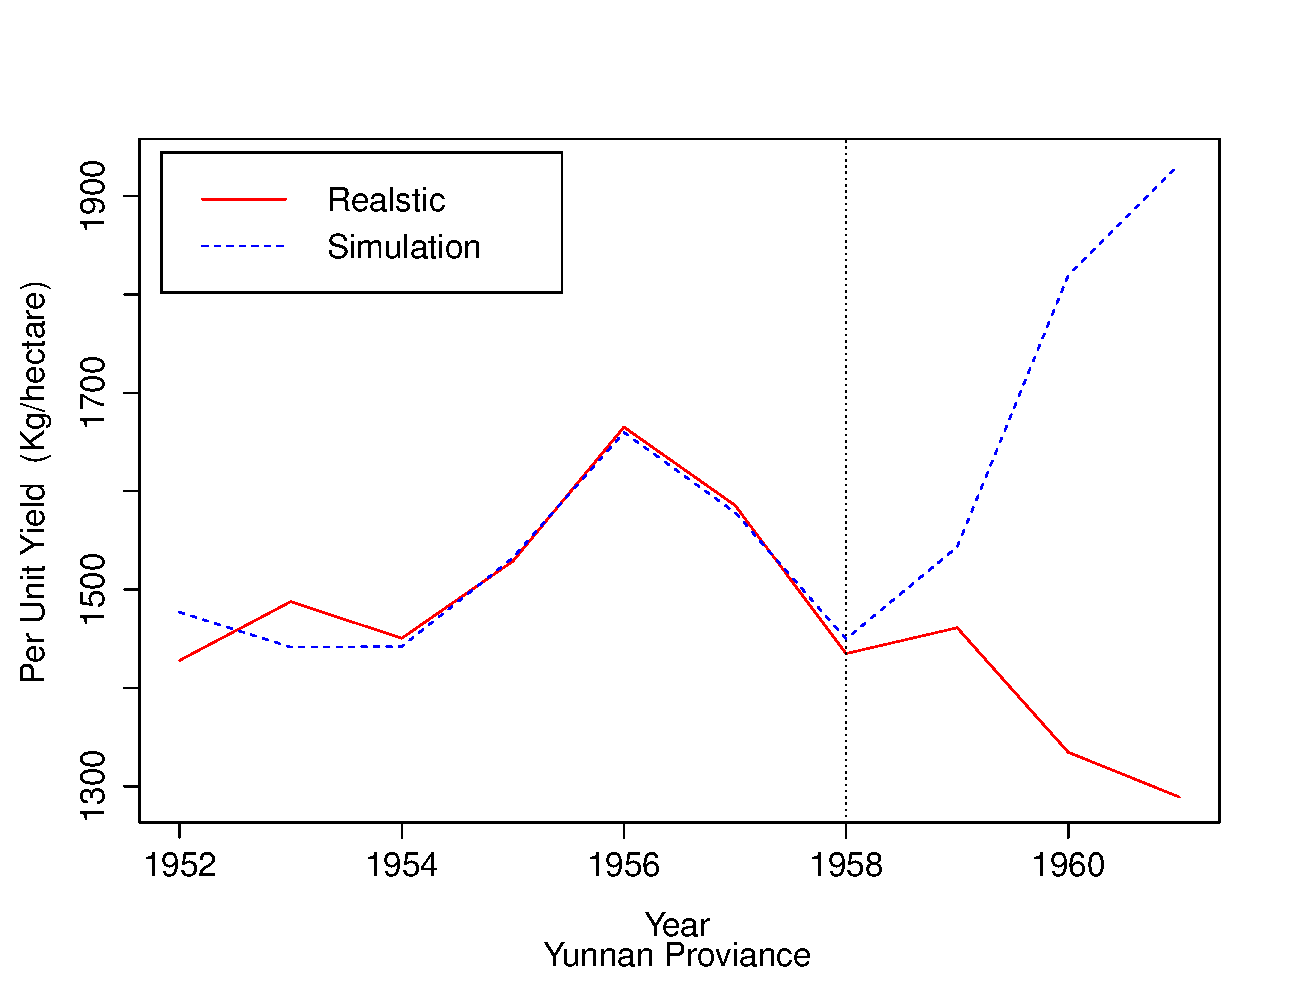
\includegraphics[width=0.7\textwidth]{images/Rplot02.eps}
\end{center}



\end{frame}


%%%%%%%%%%%%%%%%%%%%%%%%%%%%%%%%%%%%%%%%%%%%%%%%%%%%%%%%%%%%%%%%%%%%%%%%%%%%%%%%%%%%%%%%%%


%%%%%%%%%%%%%%%%%%%%%%%%%%%%%%%%%%%%%%%%%%%%%%%%%%%%%%%%%%%%%%%%%%%%%%%%%%%%%%%%%%%%%%%%%%
\section{展望}
%%%%%%%%%%%%%%%%%%%%%%%%%%%%%%%%%%%%%%%%%%%%%%%%%%%%%%%%%%%%%%%%%%%%%%%%%%%%%%%%%%%%%%%%%%
\begin{frame} 
\frametitle{Further Work}
\begin{itemize}
\item Work one
\item Work two
\item Work three

\end{itemize}
 \end{frame}

%%%%%%%%%%%%%%%%%%%%%%%%%%%%%%%%%%%%%%%%%%%%%%%%%%%%%%%%%%%%%%%%%%%%%%%%%%%%%%%%%%%%%%%%%%

\begin{frame} 
%\frametitle{The Last Slide}

\begin{center}
\huge
谢谢
\end{center}
 \end{frame}

%%%%%%%%%%%%%%%%%%%%%%%%%%%%%%%%%%%%%%%%%%%%%%%%%%%%%%%%%%%%%%%%%%%%%%%%%%%%%%%%%%%%%%%%%%
\end{document}
%%%%%%%%%%%%%%%%%%%%%%%%%%%%%%%%%%%%%%%%%%%%%%%%%%%%%%%%%%%%%%%%%%%%%%%%%%%%%%%%%%%%%%%%%%